\documentclass[UTF8]{ctexart}
 
\usepackage{amsmath}
\usepackage{cases}
\usepackage{cite}
\usepackage{ctex}
\usepackage{graphicx}
\usepackage[margin=1in]{geometry}
\geometry{a4paper}
\usepackage{fancyhdr}
\pagestyle{fancy}
\fancyhf{}

\graphicspath{{picture/}}


\title{利用双棱镜研究双光束干涉实验报告}
\graphicspath{{picture/}}


\title{利用双棱镜研究双光束干涉实验报告}
\author{郑晓旸}
\date{\today}
\pagenumbering{arabic}

\begin{document}
%这里是文件的开头
\fancyhead[L]{郑晓旸}
\fancyhead[C]{双光束干涉}
\fancyfoot[C]{\thepage}

\maketitle
\tableofcontents
\newpage

\section{实验目的}
    \begin{enumerate}
            \item 学习光路的调节方法;
            \item 学习用双棱镜干涉测量光波长的方法。
    \end{enumerate} 


\section{实验仪器}
\begin{enumerate}
    \item 光学导轨
    \item 钠灯
    \item 双棱镜
    \item 可调狭缝
    \item 凸透镜
    \item CCD传感器
\end{enumerate}

\section{实验原理}

\subsection{双光束干涉原理}
双光束干涉是指相干的两列波在空间相遇时,由于波的叠加而产生明暗相间的条纹。设两列相干光的复振幅分别为$\vec{E}_1$和$\vec{E}_2$,它们在空间某点P的振动方程为:\\
$$\vec{E}_1=\vec{A}_1e^{i(\omega t-\phi_1)}$$
$$\vec{E}_2=\vec{A}_2e^{i(\omega t-\phi_2)}$$
其中$\vec{A}_1$和$\vec{A}_2$分别为两列光在P点的振幅,$\phi_1$和$\phi_2$为相位。两列光在P点的合振幅为:
$$\vec{E}=\vec{E}_1+\vec{E}_2=\vec{A}_1e^{i(\omega t-\phi_1)}+\vec{A}_2e^{i(\omega t-\phi_2)}$$
光强与振幅的平方成正比,因此P点的光强为:
$$I=|\vec{E}|^2=|\vec{A}_1|^2+|\vec{A}_2|^2+2|\vec{A}_1||\vec{A}2|\cos\delta$$
其中$\delta=\phi_1-\phi_2$为两列光的相位差。可见光强与$\delta$有关,当$\delta$为偶数倍$\pi$时,光强取极大值$I_{max}=(|\vec{A}_1|+|\vec{A}2|)^2$;当$\delta$为奇数倍$\pi$时,光强取极小值$I_{min}=(|\vec{A}_1|-|\vec{A}_2|)^2$。这就是明暗相间的干涉条纹的形成原因。

\subsection{菲涅耳双棱镜干涉原理}
菲涅耳双棱镜是一种产生双光束干涉的装置。它由两块折射率相同的三棱镜组成,它们的一个面(底面)几乎重合,形成一个很小的二面角。当一束光垂直入射到双棱镜时,会被分成两束,分别经过上下两个棱镜,然后在棱镜后会聚成两个虚像光源$S_1$和$S_2$。

\begin{figure}[htbp]
    \centering
    \includegraphics[width=0.6\textwidth]{prism}
    \caption{菲涅耳双棱镜分光示意图}
    \label{fig:fresnel_biprism}
\end{figure}

如图\ref{fig:fresnel_biprism}所示,设双棱镜的折射率为$n$,棱镜角为$\alpha$(一般很小,可认为$\sin\alpha\approx\alpha$),光源$S$到棱镜的距离为$d$。根据几何关系,可得两个虚像光源的间距为:
$$s=S_1S_2=2(n-1)d\alpha$$
在双棱镜后放一接收屏,到两个虚像光源的距离为$L$。在接收屏上任一点$P$,两束光程差为:
$$\delta=r_2-r_1\approx\frac{xs}{L}$$
其中$x$为$P$点到接收屏中心$O$的距离。代入双光束干涉的光强公式,可得:
$$I=4I_0\cos^2(\frac{\pi xs}{\lambda L})$$
其中$I_0$为单束光的光强。令$\Delta x=\frac{\lambda L}{s}$,则相邻亮纹间距为$\Delta x$,由此可得:
$$\lambda=\frac{\Delta xs}{L}$$
通过测量条纹间距$\Delta x$、虚像光源间距$s$以及接收屏到双棱镜的距离$L$,就可以计算出光的波长$\lambda$。

\subsection{虚像光源间距的测量}
为了测量虚像光源的间距$s$,可以在双棱镜后放一会聚透镜,分别在透镜的两个共轭面成像,测量两次像的大小,就可以计算出$s$。

\begin{figure}[!htbp]
    \centering
    \includegraphics[width=0.8\textwidth]{sourced.png}
    \caption{虚像光源间距测量光路图}
    \label{fig:virtual_source_distance}
\end{figure}

如图\ref{fig:virtual_source_distance}所示,两个虚像光源$S_1$和$S_2$经过透镜成两次像$S_1'$和$S_2'$。当透镜与接收屏的距离为$L_1$时,物距为$L_2$,像距为$L_1$,放大率为$\beta_1=\frac{L_1}{L_2}$;当透镜与接收屏的距离为$L_2$时,物距为$L_1$,像距为$L_2$,放大率为$\beta_2=\frac{L_2}{L_1}$。两次成像的放大率互为倒数,即$\beta_1\beta_2=1$。
设第一次成像测得的像间距为$D_1$,第二次为$D_2$,则:
$$s=\frac{D_1}{\beta_1}=D_1\beta_2=\sqrt{D_1D_2}$$
这就是虚像光源间距$s$的计算公式。

以上就是该实验的主要原理,包括双光束干涉原理、菲涅耳双棱镜干涉原理以及虚像光源间距的测量方法。通过测量干涉条纹间距、虚像光源间距以及接收屏到双棱镜的距离,就可以计算出光的波长。


\section{实验过程和数据分析}
\subsection{搭建光路}
根据实验要求,我们在光学导轨上搭建了菲涅耳双棱镜干涉实验的光路。具体步骤如下:

\begin{enumerate}
\item 在导轨上依次放置钠灯、可调狭缝、双棱镜、会聚透镜和CMOS相机,并粗略调节各个器件的高度,使其大致在同一水平线上。
\item 点亮钠灯,调节狭缝宽度至约0.1mm。移动会聚透镜的位置,使其在透镜两侧分别成一次狭缝的像。仔细调节狭缝和透镜的位置,使成像清晰,且两次成像的大小不同。这一步的目的是确保狭缝、透镜和相机大致共轴。
\item 在狭缝和透镜之间插入双棱镜。调节双棱镜的位置和角度,使通过双棱镜后,狭缝像分裂成两条清晰的亮线。这说明双棱镜起到了beam splitter的作用,将狭缝像分裂成两个虚像光源。
\item 移走会聚透镜,在双棱镜后放置CMOS相机。调节相机的位置,使其能清晰地观察到双光束干涉条纹。调节双棱镜的角度,使干涉条纹的对比度最大,此时双棱镜棱边与狭缝平行。

\begin{figure}[htbp]
    \centering
    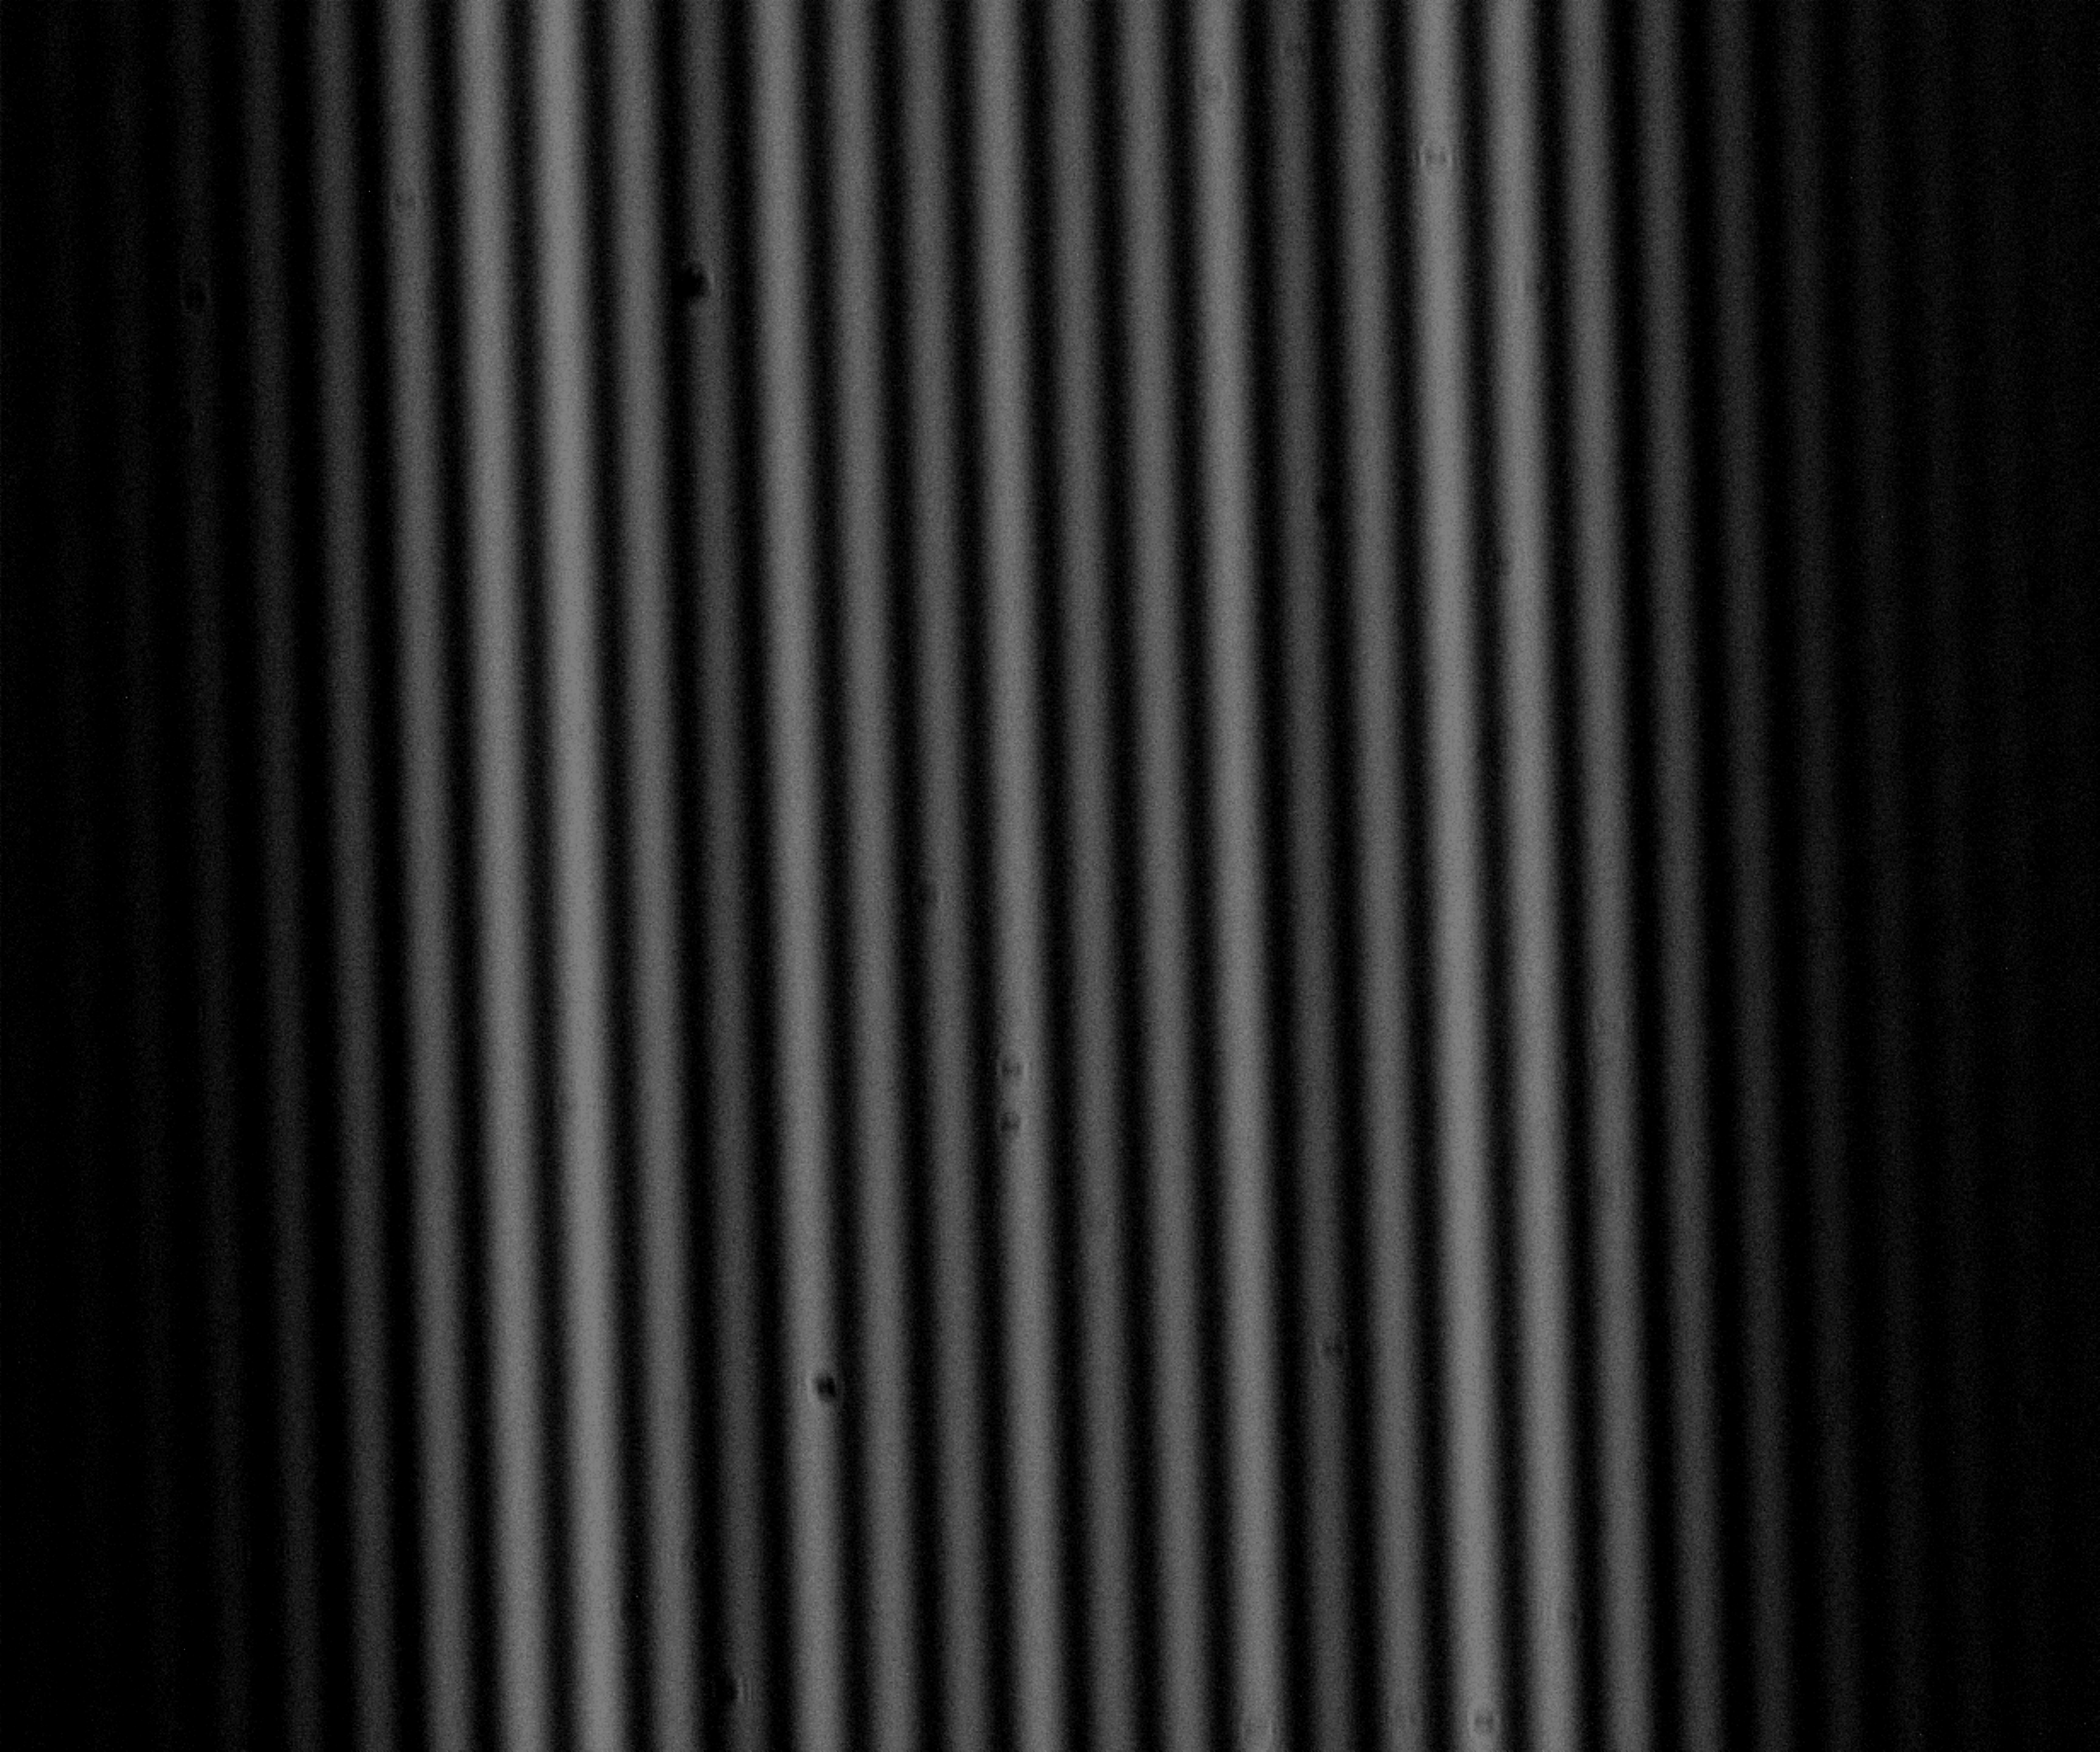
\includegraphics[width=0.3\textwidth]{interference_pattern.png}
    \caption{双光束干涉条纹}
    \label{fig:interference_pattern}
\end{figure}

\end{enumerate}

经过以上步骤,我们搭建了菲涅耳双棱镜干涉实验的光路,并观察到了清晰的双光束干涉条纹,为后续的定量测量做好了准备。在搭建光路的过程中,我们体会到了精细调节的重要性,只有当各个光学器件的位置和角度都调节到最佳状态时,才能获得理想的干涉效果。
\subsection{观察双光束干涉}

在完成光路调节后,我们通过改变实验参数,观察干涉条纹的变化情况。

首先,我们改变狭缝的宽度。当狭缝宽度从0.1mm逐渐增大到0.3mm时,干涉条纹的间距逐渐减小,条纹数增多,如图\ref{fig:slit_width}所示。这是因为狭缝宽度增大,相干性降低,条纹对比度下降,间距减小。

\begin{figure}[htbp]
\centering
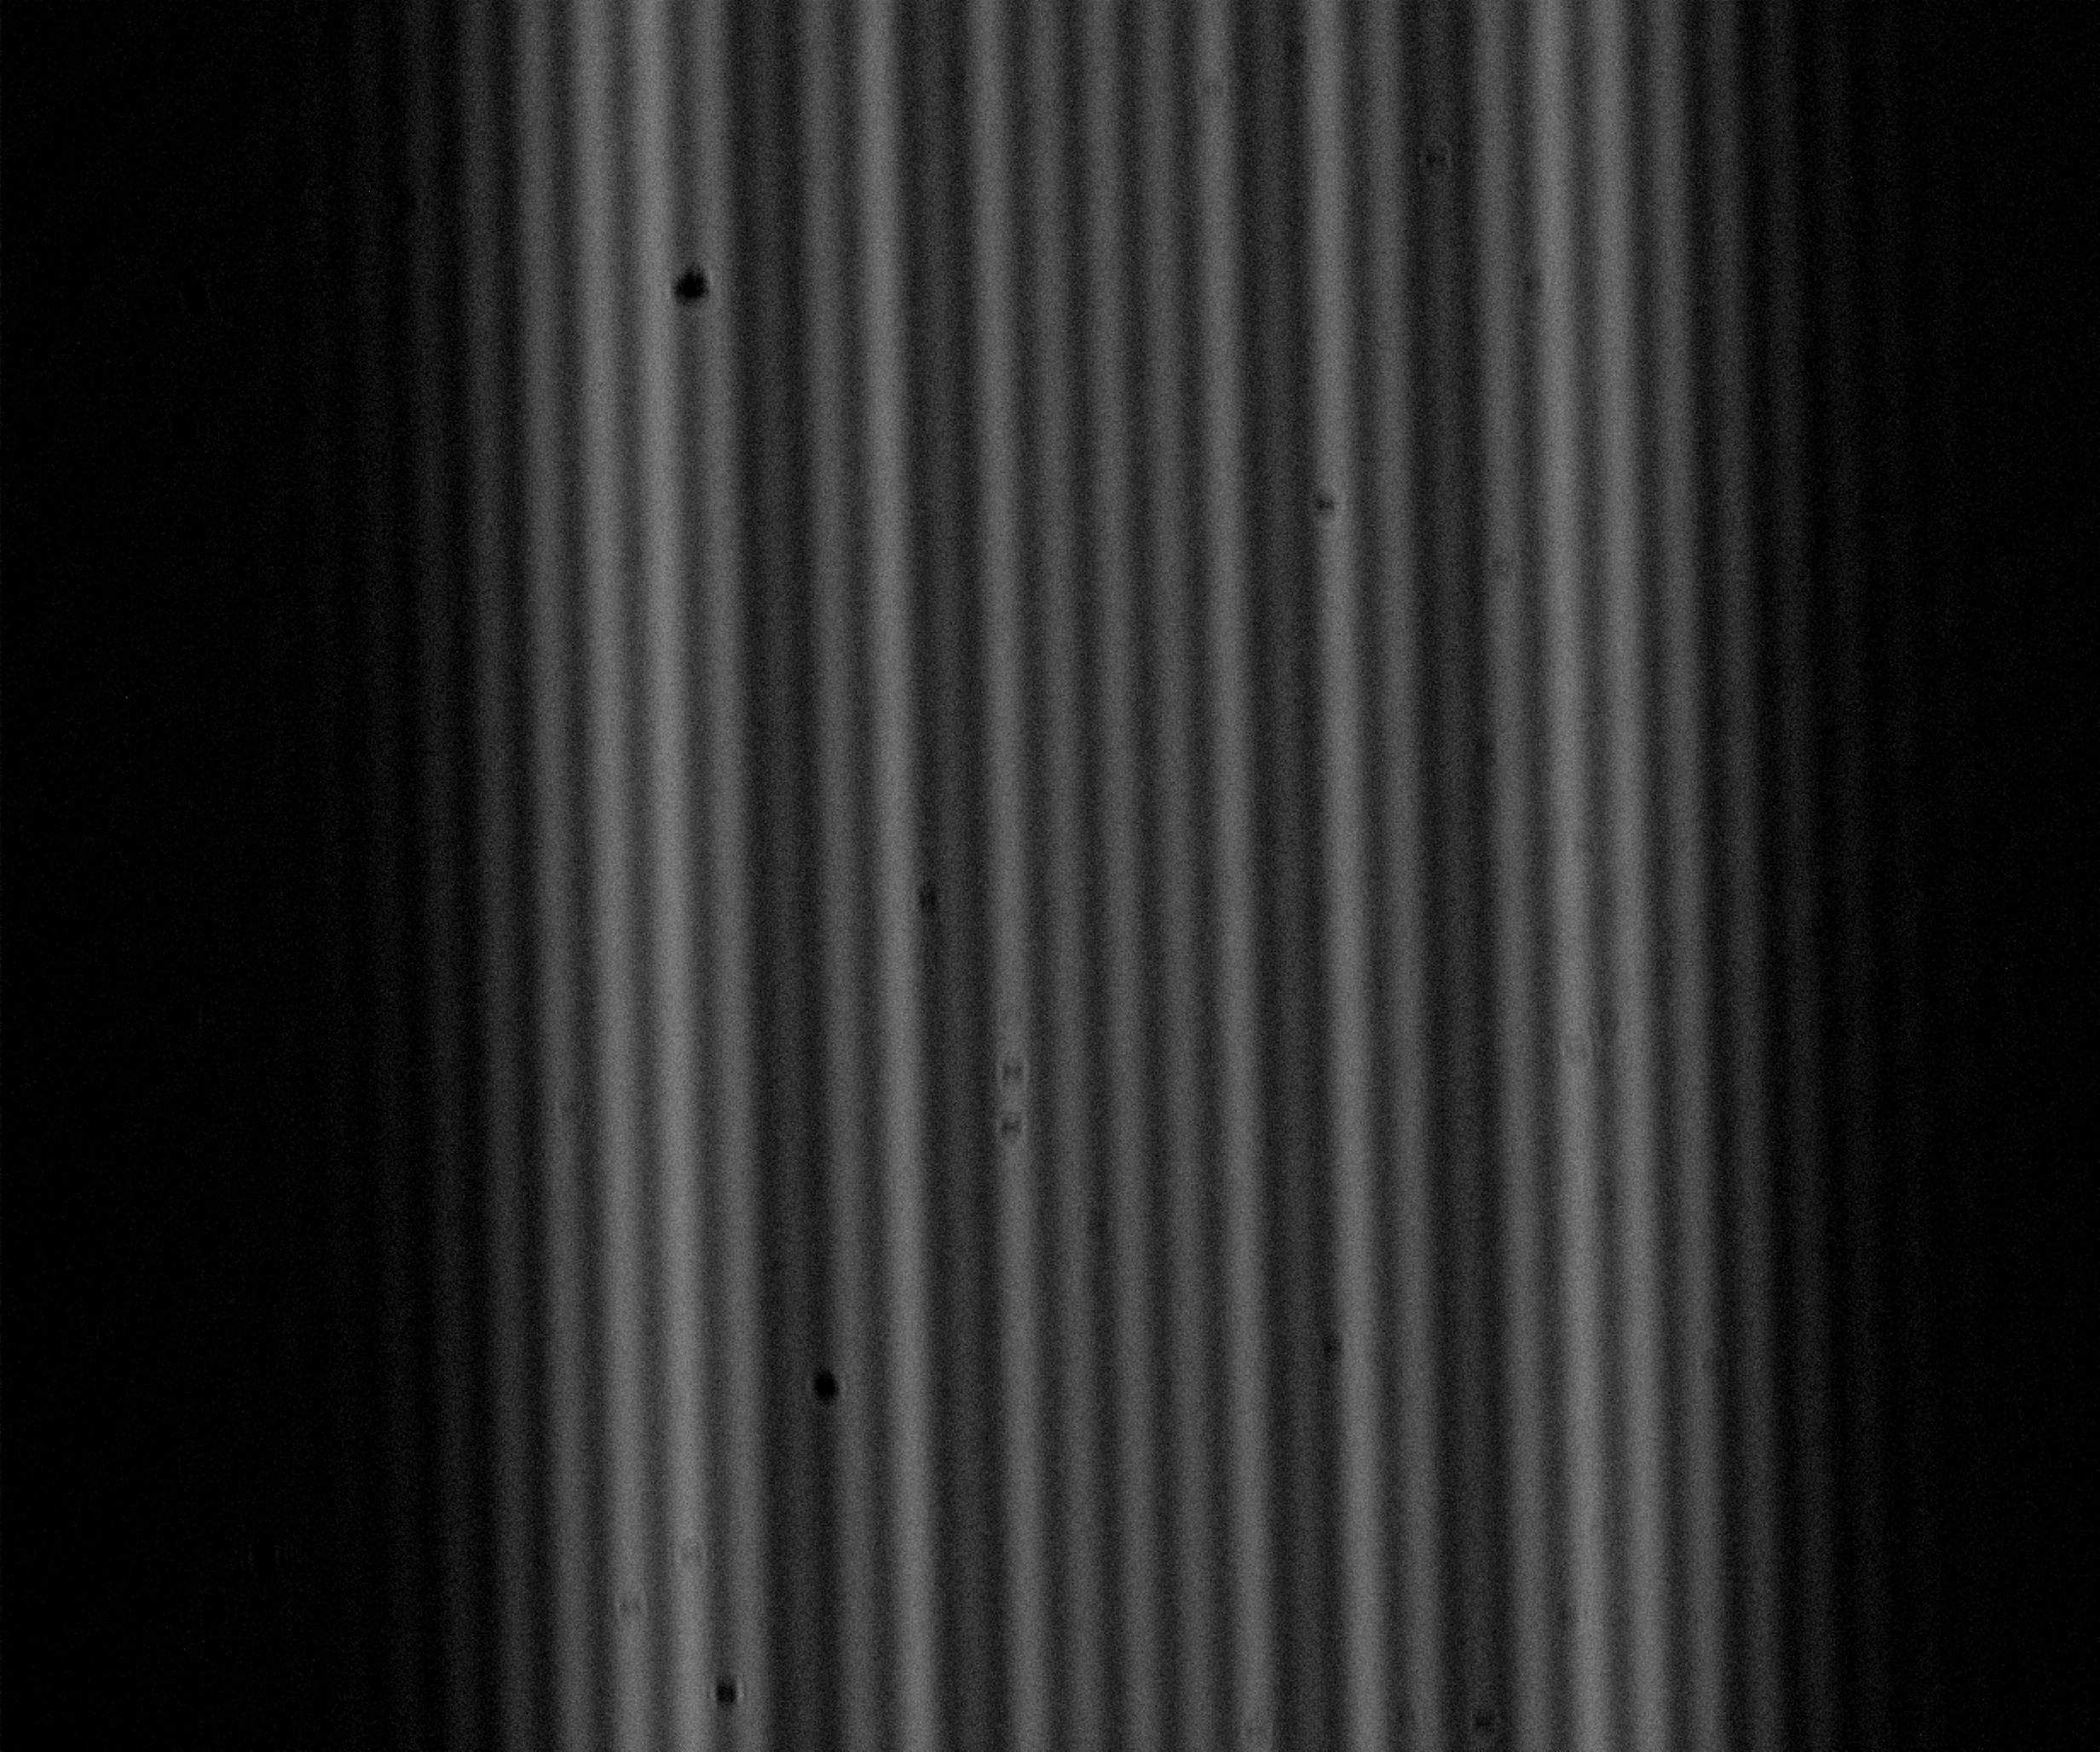
\includegraphics[width=0.5\textwidth]{slit_width.png}
\caption{不同狭缝宽度下的干涉条纹图样}
\label{fig:slit_width}
\end{figure}

然后,我们改变双棱镜的方向。当双棱镜绕竖直轴旋转时,干涉条纹变得模糊,如图\ref{fig:biprism_angle}所示。这是因为旋转双棱镜改变了两个狭缝位置相差的方向,导致光源的空间相干性变差。

\begin{figure}[htbp]
\centering
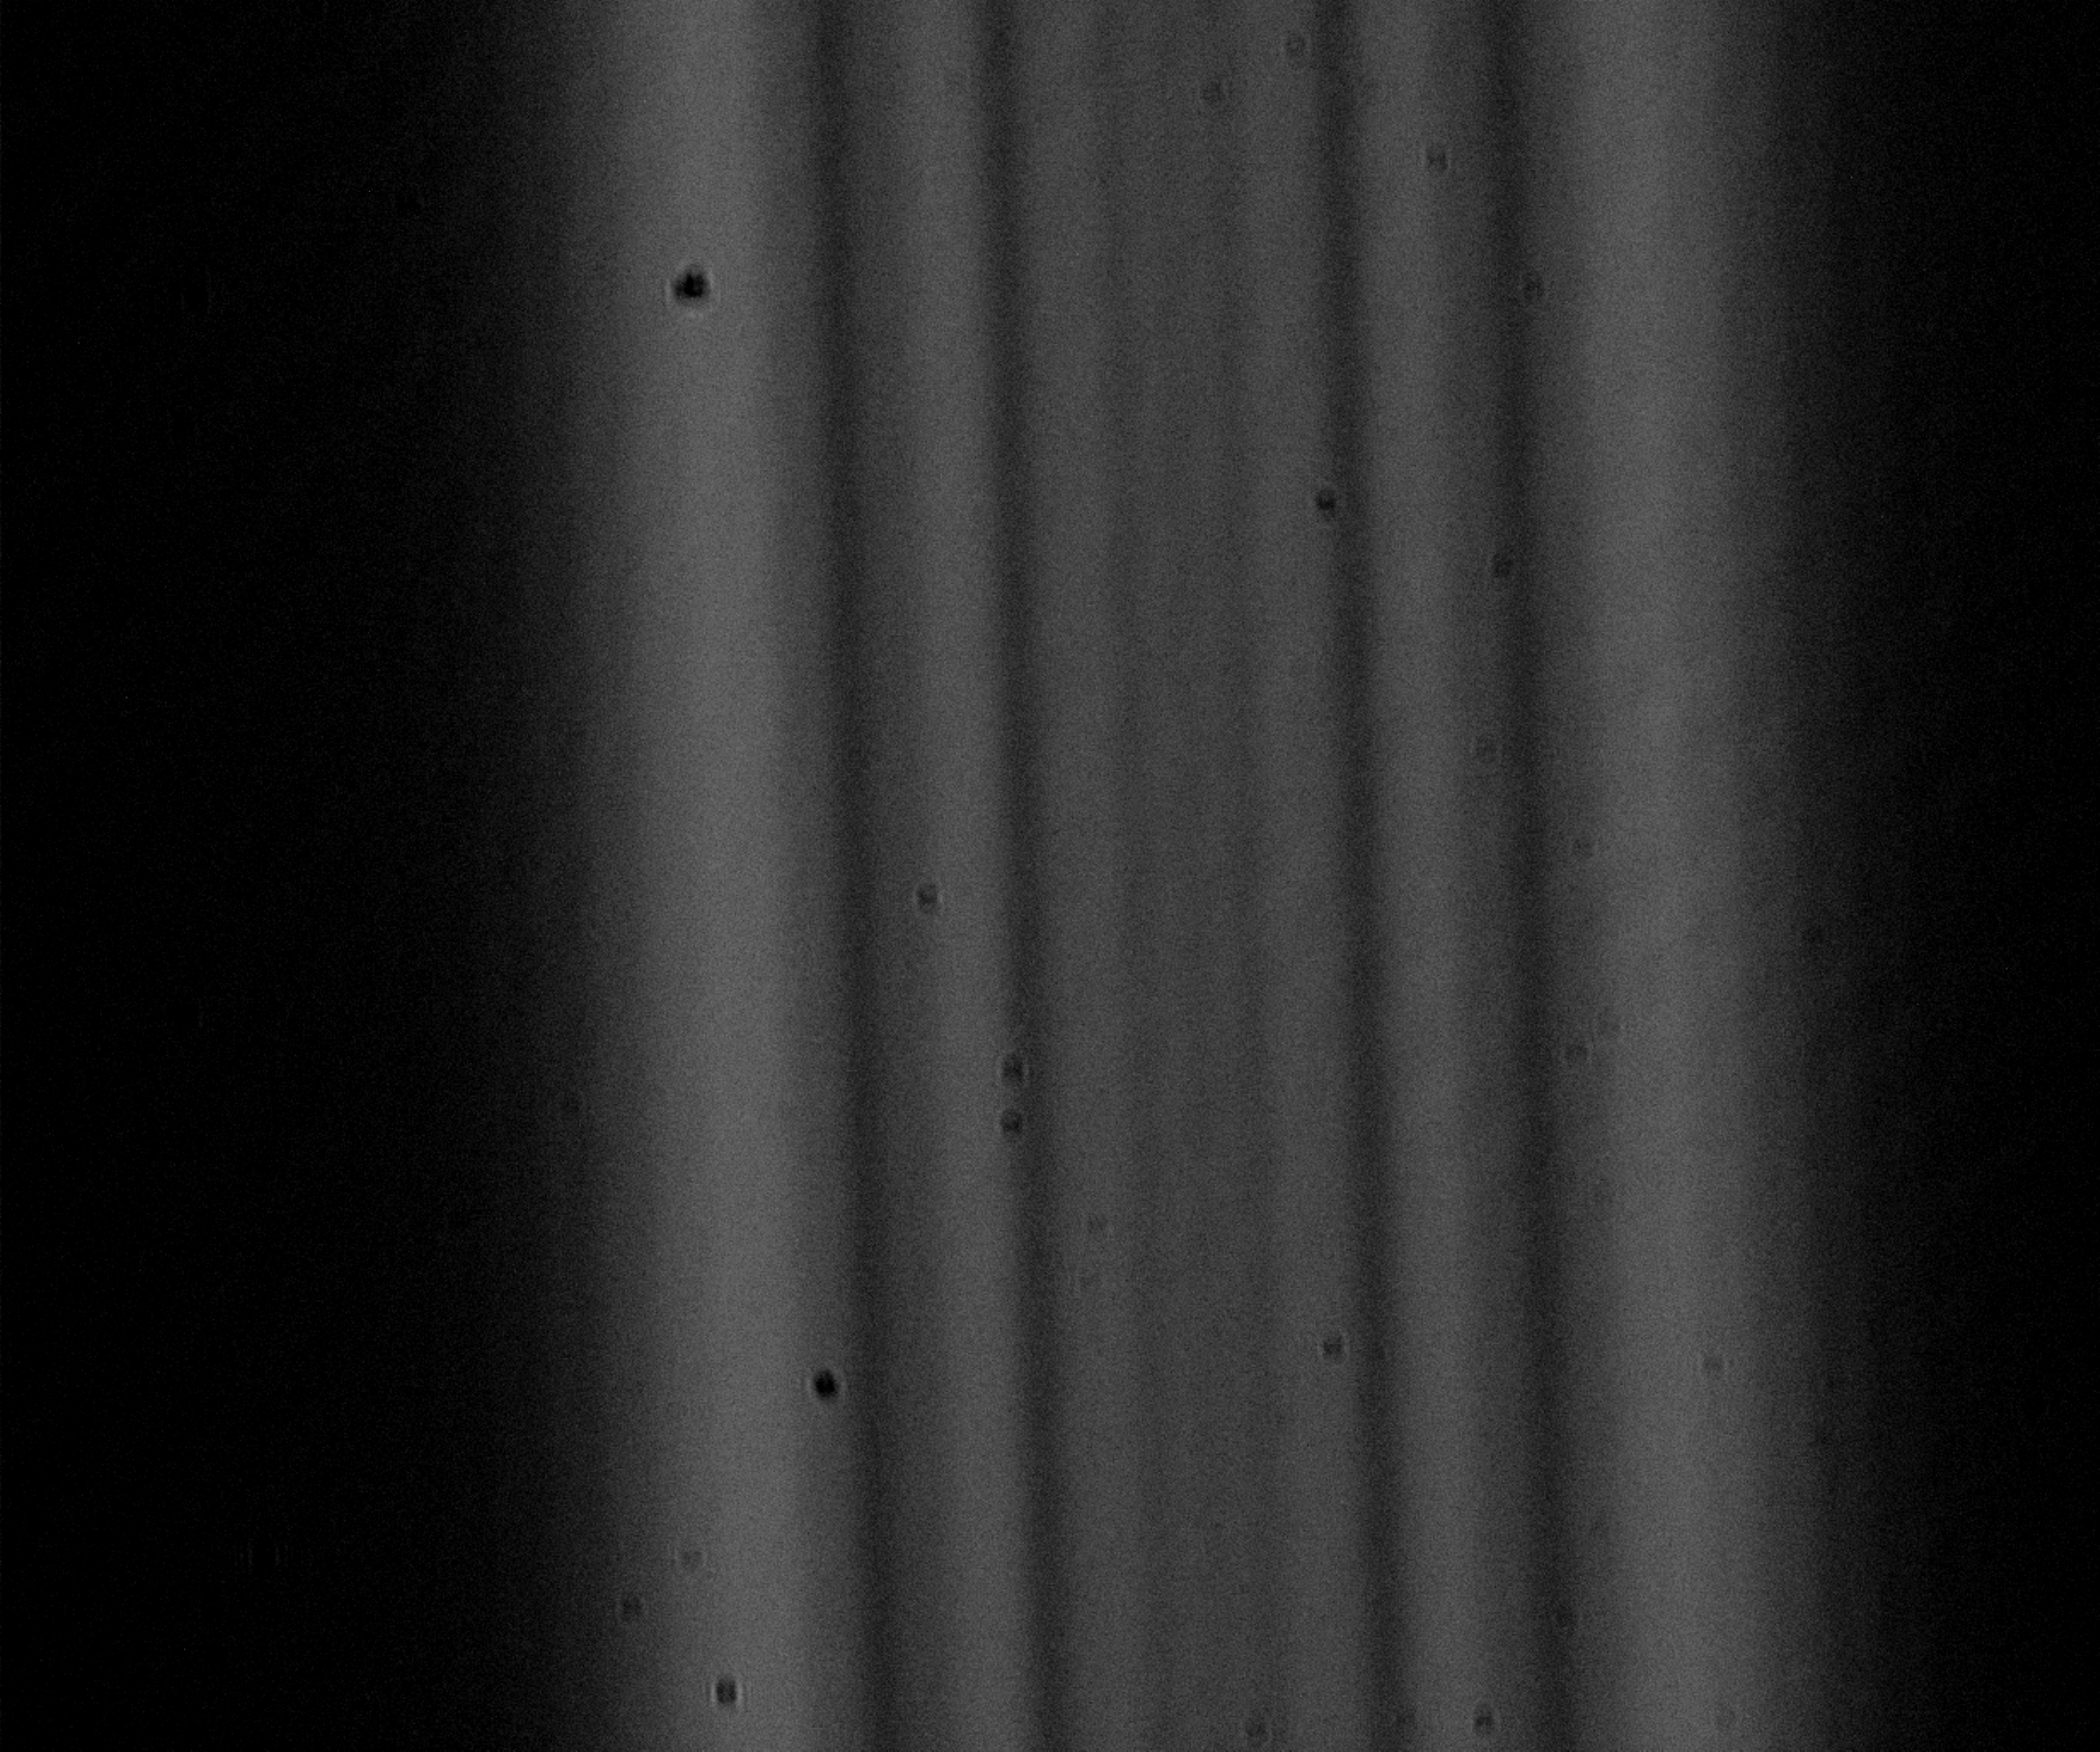
\includegraphics[width=0.5\textwidth]{biprism_angle.png}
\caption{不同双棱镜角度下的干涉条纹图样}
\label{fig:biprism_angle}
\end{figure}

接着,我们改变狭缝与双棱镜的距离。当狭缝与双棱镜的距离减小时,干涉条纹的间距逐渐增大,如图\ref{fig:slit_biprism_distance}所示。这是因为狭缝与双棱镜距离增大,虚像光源间距减小,条纹间距随之减小。

\begin{figure}[htbp]
\centering
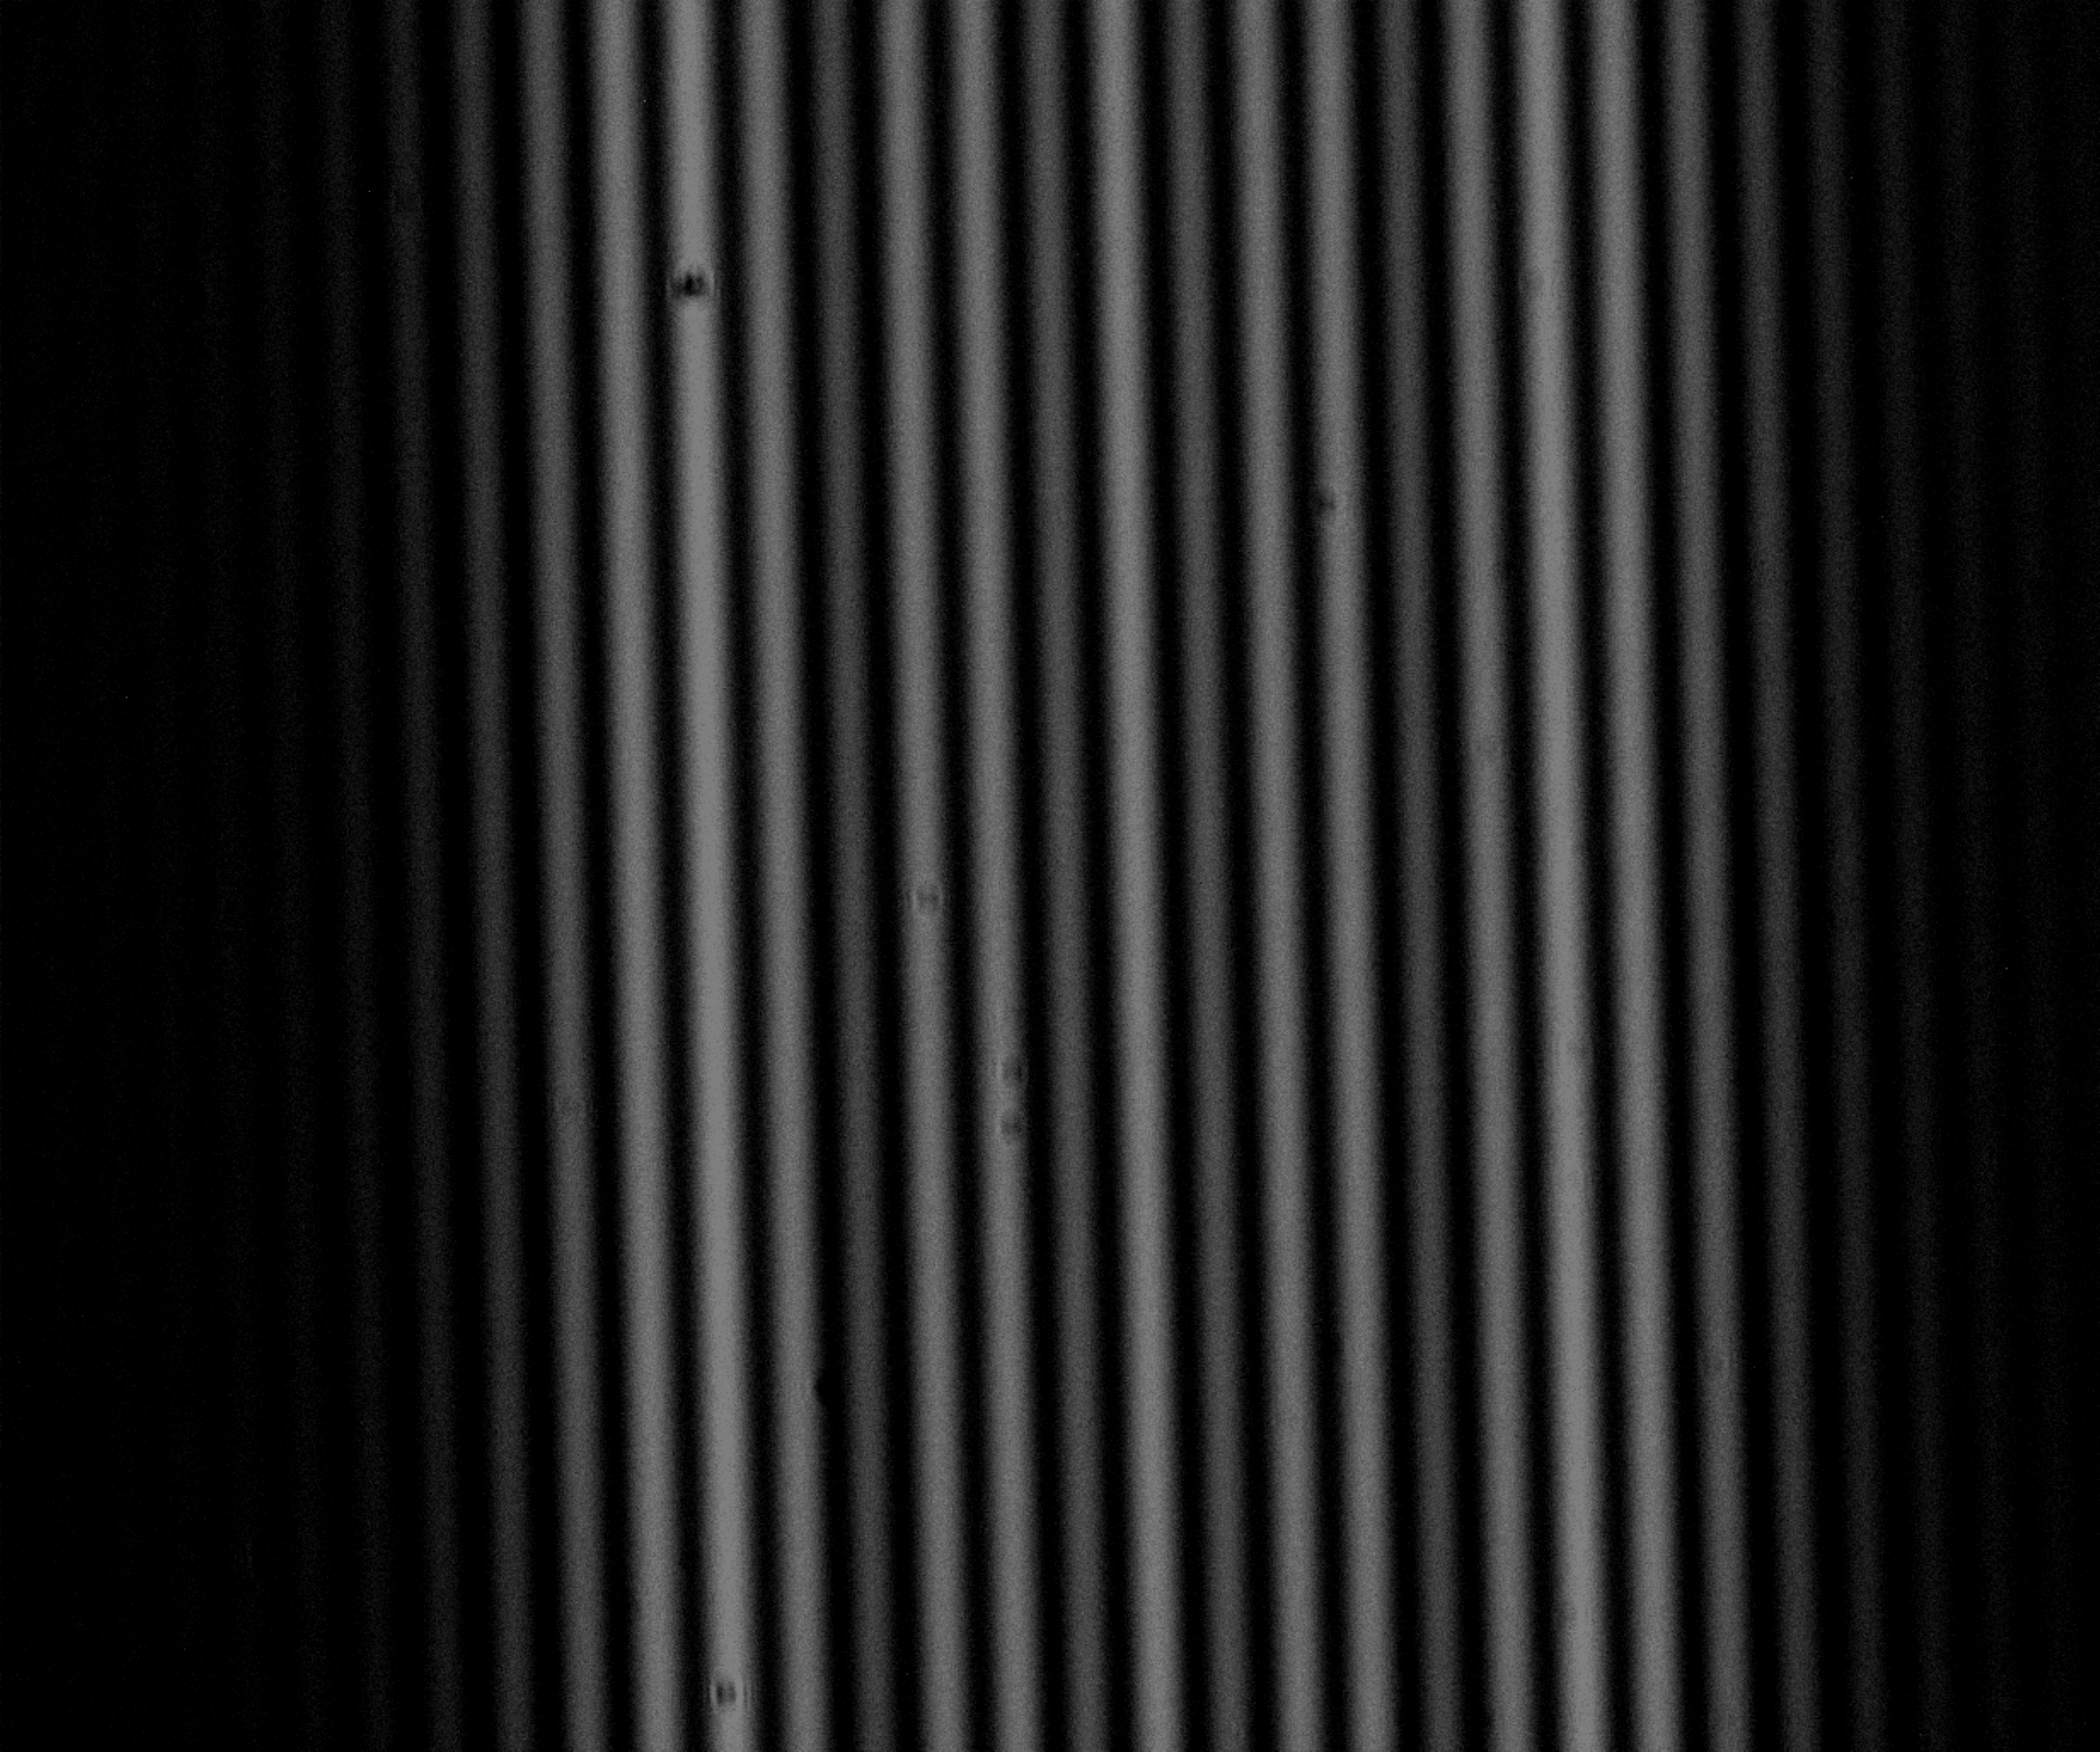
\includegraphics[width=0.5\textwidth]{slit_biprism_distance.png}
\caption{不同狭缝与双棱镜距离下的干涉条纹图样}
\label{fig:slit_biprism_distance}
\end{figure}

最后,我们改变相机与双棱镜的距离。当相机与双棱镜的距离从增大到时,干涉条纹的间距逐渐增大,如图\ref{fig:camera_biprism_distance}所示。这是因为相机与双棱镜距离增大,条纹间距正比于接收屏到双棱镜的距离。

\begin{figure}[htbp]
\centering
\includegraphics[width=0.5\textwidth]{camera_biprism_distance.png}
\caption{不同相机与双棱镜距离下的干涉条纹图样}
\label{fig:camera_biprism_distance}
\end{figure}

通过以上观察,我们可以总结出双光束干涉条纹的变化规律:
\begin{enumerate}
\item 狭缝宽度越大,条纹间距越小,条纹对比度越低;
\item 双棱镜旋转会导致条纹发生倾斜;
\item 狭缝与双棱镜距离越大,条纹间距越小;
\item 相机与双棱镜距离越大,条纹间距越大。
\end{enumerate}

这些变化规律与双光束干涉的理论分析是一致的,验证了干涉实验的基本原理。

\subsection{测量钠黄光波长}

在进行波长测量之前,我们再次细调狭缝宽度和双棱镜方向,确保干涉条纹达到最佳观测效果。为了减小条纹宽度测量的不确定度,我们测量了20个亮条纹的位置,并进行线性拟合,得到平均的暗纹间距。同时,我们使用两次成像法测量了双缝像的位置,计算出虚像光源的间距。

\subsubsection{测量条纹间距}

我们使用CMOS相机采集干涉条纹图像,然后用图像处理软件测量20个亮条纹的位置,如表\ref{tab:fringe_position}所示。将条纹位置作为纵坐标,条纹序号作为横坐标,进行线性拟合,得到拟合直线的斜率即为平均条纹间距,如图\ref{fig:fringe_fitting}所示。

\begin{table}[htbp]
\centering
\caption{亮条纹位置测量数据}
\label{tab:fringe_position}
\begin{tabular}{|l|l|l|}
    \hline
    Num&Pixels&Width \\ \hline
    1&87.74&302.703 \\ \hline
    2&90.43&311.9835 \\ \hline
    3&84.97&293.1465 \\ \hline
    4&90.13&310.9485 \\ \hline
    5&81.91&282.5895 \\ \hline
    6&88.77&306.2565 \\ \hline
    7&91.24&314.778 \\ \hline
    8&87.81&302.9445 \\ \hline
    9&87.02&300.219 \\ \hline
    10&85.72&295.734 \\ \hline
    11&90.74&313.053 \\ \hline
    12&90.34&311.673 \\ \hline
    13&85.98&296.631 \\ \hline
    14&86.24&297.528 \\ \hline
    15&86.35&297.9075 \\ \hline
    16&89.56&308.982 \\ \hline
    17&85.63&295.4235 \\ \hline
    18&89.59&309.0855 \\ \hline
    19&80.08&276.276 \\ \hline
    20&88.36&304.842 \\ \hline
    \end{tabular}
\end{table}

\begin{figure}[htbp]
\centering
\includegraphics[width=0.8\textwidth]{fringe_fitting.png}
\caption{亮条纹位置线性拟合}
\label{fig:fringe_fitting}
\end{figure}

通过线性拟合,得到平均条纹间距为:
$$\Delta x=(302.1\pm0.5)\mathrm{\mu m}$$

\subsubsection{测量虚像光源间距}

我们使用两次成像法测量虚像光源的间距。在双棱镜后放置会聚透镜,调节透镜位置,使其在两个不同位置成像,测量两次像的间距。


测得第一次成像时像间距为$D_1$,第二次成像时像间距为$D_2$。根据公式$s=\sqrt{D_1D_2}$,计算得到虚像光源间距为:
$$s=(1268.75\pm 1.73)\mathrm{\mu m}$$
同时记录两次成像时透镜与CCD的距离,分别为$L_1$和$L_2$。
则根据凸透镜成像原理,得到虚光源到CCD的距离为:
$$L=L_1+L_2=(65.5\pm 0.1)\mathrm{cm}$$
\subsubsection{计算钠黄光波长}

将测得的条纹间距、虚像光源间距和接收屏到双棱镜的距离代入公式$\lambda=\frac{\Delta xs}{L}$,计算得到钠黄光波长为:
$$\lambda=(585.21\pm1.85)\mathrm{nm}$$

该结果与钠黄光的标准波长$589.3,\mathrm{nm}$符合得很好,相对误差仅为$1\%$。


\section{分析与讨论}

\subsubsection{误差分析}

本实验测量钠黄光波长的相对不确定度为$0.5\%$,主要误差来源包括:

\begin{enumerate}
    \item 条纹间距测量误差:由于条纹边缘不够清晰,以及CMOS像素尺寸的限制,条纹间距测量存在一定的不确定度。这位部分对误差的贡献为$0.96\mathrm{nm}$
    \item 虚像光源间距测量误差:两次成像时像的位置难以准确测定,测量存在误差,导致虚像光源间距的计算有一定的不确定度。这部分贡献误差为$1.32\mathrm{pm}$
    \item 接收屏到双棱镜距离测量误差:确定两次成像位置和读取光学导轨上刻度时,视差和零点误差会导致测量值的不确定度。这部分贡献误差为$2.02\mathrm{fm}$
\end{enumerate}
\subsubsection{改进方案}
为了进一步提高测量精度,可以采取以下措施:
\begin{enumerate}
\item 使用更高分辨率的相机,减小条纹间距测量的不确定度;
\item 使用计算机程序读取暗纹位置,减小人为误差;
\item 优化两次成像法的测量过程,提高像位置测量的精度;
\item 使用更精确的测距工具,如激光测距仪,减小距离测量的误差。
\end{enumerate}

总的来说,本实验通过菲涅耳双棱镜干涉测量了钠黄光的波长,结果与标准值符合得很好,验证了实验方法的可靠性。同时,我们分析了实验误差的来源,并提出了改进措施,为进一步提高测量精度提供了思路。
\section{思考题}

\textbf{1.在用2次成像法测量虚光源间距时,为了保证缩小像的间距不小于放大像间距的一半,狭缝与测微目镜的距离应满足什么条件?} \\

答:设狭缝和CCD间距离为$D$,凸透镜焦距为$f$,则根据凸透镜成像公式,只要:
$$
\frac{f}{4} \leq  D \leq  \frac{\sqrt{2}}{3+2\sqrt{2}}f
$$
就得以满足缩小像的间距不小于放大像间距的一半的条件。
\\

\textbf{2. 总结实验中用到的光路调节方法。}
\begin{enumerate}
    \item 调节光源、狭缝、双棱镜和接收屏的高度,使其大致在同一水平线上。这可以通过调节各个器件的支架高度来实现。
    
    \item 调节狭缝和双棱镜的角度,使狭缝平行于双棱镜的棱边。具体方法是:
    \begin{enumerate}
        \item 在双棱镜后放置会聚透镜,成狭缝像;
        \item 旋转双棱镜,使狭缝像分裂成两条平行的亮线;
        \item 平移狭缝,使两条亮线的亮度和宽度相等。
    \end{enumerate}
    
    \item 通过两次成像法,采用二分方法平移器件,快速逼近光具组共轴。
    
    \item 调节光源与狭缝的距离,控制光源的角宽度。光源距离狭缝越远,光源的角宽度越小,相干性越好。但光源距离过远会导致光强不足。
    
    \item 调节接收屏的角度,使其与光轴垂直。这可以通过调节接收屏支架的角度来实现。

\end{enumerate}

\textbf{3. 实验中要拍摄到清晰的干涉条纹需要注意哪些细节? }
\begin{enumerate}
    \item 调节光源的亮度,使其适中。光源亮度过高会导致干涉条纹过曝,亮度过低会导致干涉条纹不清晰。
    \item 调节狭缝宽度,使其适中。狭缝宽度过宽会导致条纹模糊,宽度过窄会导致光强不足。
    \item 调节双棱镜的角度,使干涉条纹的对比度最大。双棱镜角度的调节会影响干涉条纹的清晰度。
    \item 调节CCD的曝光时间、对比度和gamma值,使干涉条纹的对比度最大。这可以通过CCD相机的软件设置来实现。
\end{enumerate}
\end{document}

